% CVPR 2025 Paper Template; see https://github.com/cvpr-org/author-kit

\documentclass[10pt,twocolumn,letterpaper]{article}

%%%%%%%%% PAPER TYPE  - PLEASE UPDATE FOR FINAL VERSION
% \usepackage{cvpr}              % To produce the CAMERA-READY version
% \usepackage[review]{cvpr}      % To produce the REVIEW version
\usepackage[pagenumbers]{cvpr} % To force page numbers, e.g. for an arXiv version

% Import additional packages in the preamble file, before hyperref
%
% --- inline annotations
%
\newcommand{\red}[1]{{\color{red}#1}}
\newcommand{\todo}[1]{{\color{red}#1}}
\newcommand{\TODO}[1]{\textbf{\color{red}[TODO: #1]}}
% --- disable by uncommenting  
% \renewcommand{\TODO}[1]{}
% \renewcommand{\todo}[1]{#1}



% It is strongly recommended to use hyperref, especially for the review version.
% hyperref with option pagebackref eases the reviewers' job.
% Please disable hyperref *only* if you encounter grave issues, 
% e.g. with the file validation for the camera-ready version.
%
% If you comment hyperref and then uncomment it, you should delete *.aux before re-running LaTeX.
% (Or just hit 'q' on the first LaTeX run, let it finish, and you should be clear).
\definecolor{cvprblue}{rgb}{0.21,0.49,0.74}
\usepackage[pagebackref,breaklinks,colorlinks,allcolors=cvprblue]{hyperref}

%%%%%%%%% PAPER ID  - PLEASE UPDATE
\def\paperID{15557} % *** Enter the Paper ID here
\def\confName{CVPR}
\def\confYear{2025}

%%%%%%%%% TITLE - PLEASE UPDATE
\title{VMix: Improving Text-to-Image Diffusion Model \\ with
Cross-Attention Mixing Control}

%%%%%%%%% AUTHORS - PLEASE UPDATE
% \author{First Author\\
% Institution1\\
% Institution1 address\\
% {\tt\small firstauthor@i1.org}
% % For a paper whose authors are all at the same institution,
% % omit the following lines up until the closing ``}''.
% % Additional authors and addresses can be added with ``\and'',
% % just like the second author.
% % To save space, use either the email address or home page, not both
% \and
% Second Author\\
% Institution2\\
% First line of institution2 address\\
% {\tt\small secondauthor@i2.org}
% }

\author{
\textbf{Shaojin Wu$^{1}$,
Fei Ding$^1$\thanks{Corresponding author.},
Mengqi Huang$^{1,2}$,
Wei Liu$^1$,
Qian He$^1$}
\smallskip 
\\
$^1$ByteDance Inc, $^2$University of Science and Technology of China
\smallskip 
\\
\tt\small\{wushaojin, dingfei.212, liuwei.jikun, heqian\}@bytedance.com 
\tt\small\{huangmq\}@mail.ustc.edu.cn
}

\begin{document}
\maketitle
\begin{abstract}
Diffusion Models have emerged as powerful generative models for high-quality image synthesis, with many subsequent image editing techniques based on them. However, the ease of text-based image editing introduces significant risks, such as malicious editing for scams or intellectual property infringement. Previous works have attempted to safeguard images from diffusion-based editing by adding imperceptible perturbations. These methods are costly and specifically target prevalent Latent Diffusion Models (LDMs), while Pixel-domain Diffusion Models (PDMs) remain largely unexplored and robust against such attacks. Our work addresses this gap by proposing a novel attacking framework with a feature representation attack loss that exploits vulnerabilities in denoising UNets and a latent optimization strategy to enhance the naturalness of protected images. Extensive experiments demonstrate the effectiveness of our approach in attacking dominant PDM-based editing methods (e.g., SDEdit) while maintaining reasonable protection fidelity and robustness against common defense methods. Additionally, our framework is extensible to LDMs, achieving comparable performance to existing approaches.
\end{abstract}
    
\section{Introduction}
\label{sec:intro}

\begin{figure*}[t]
\centering
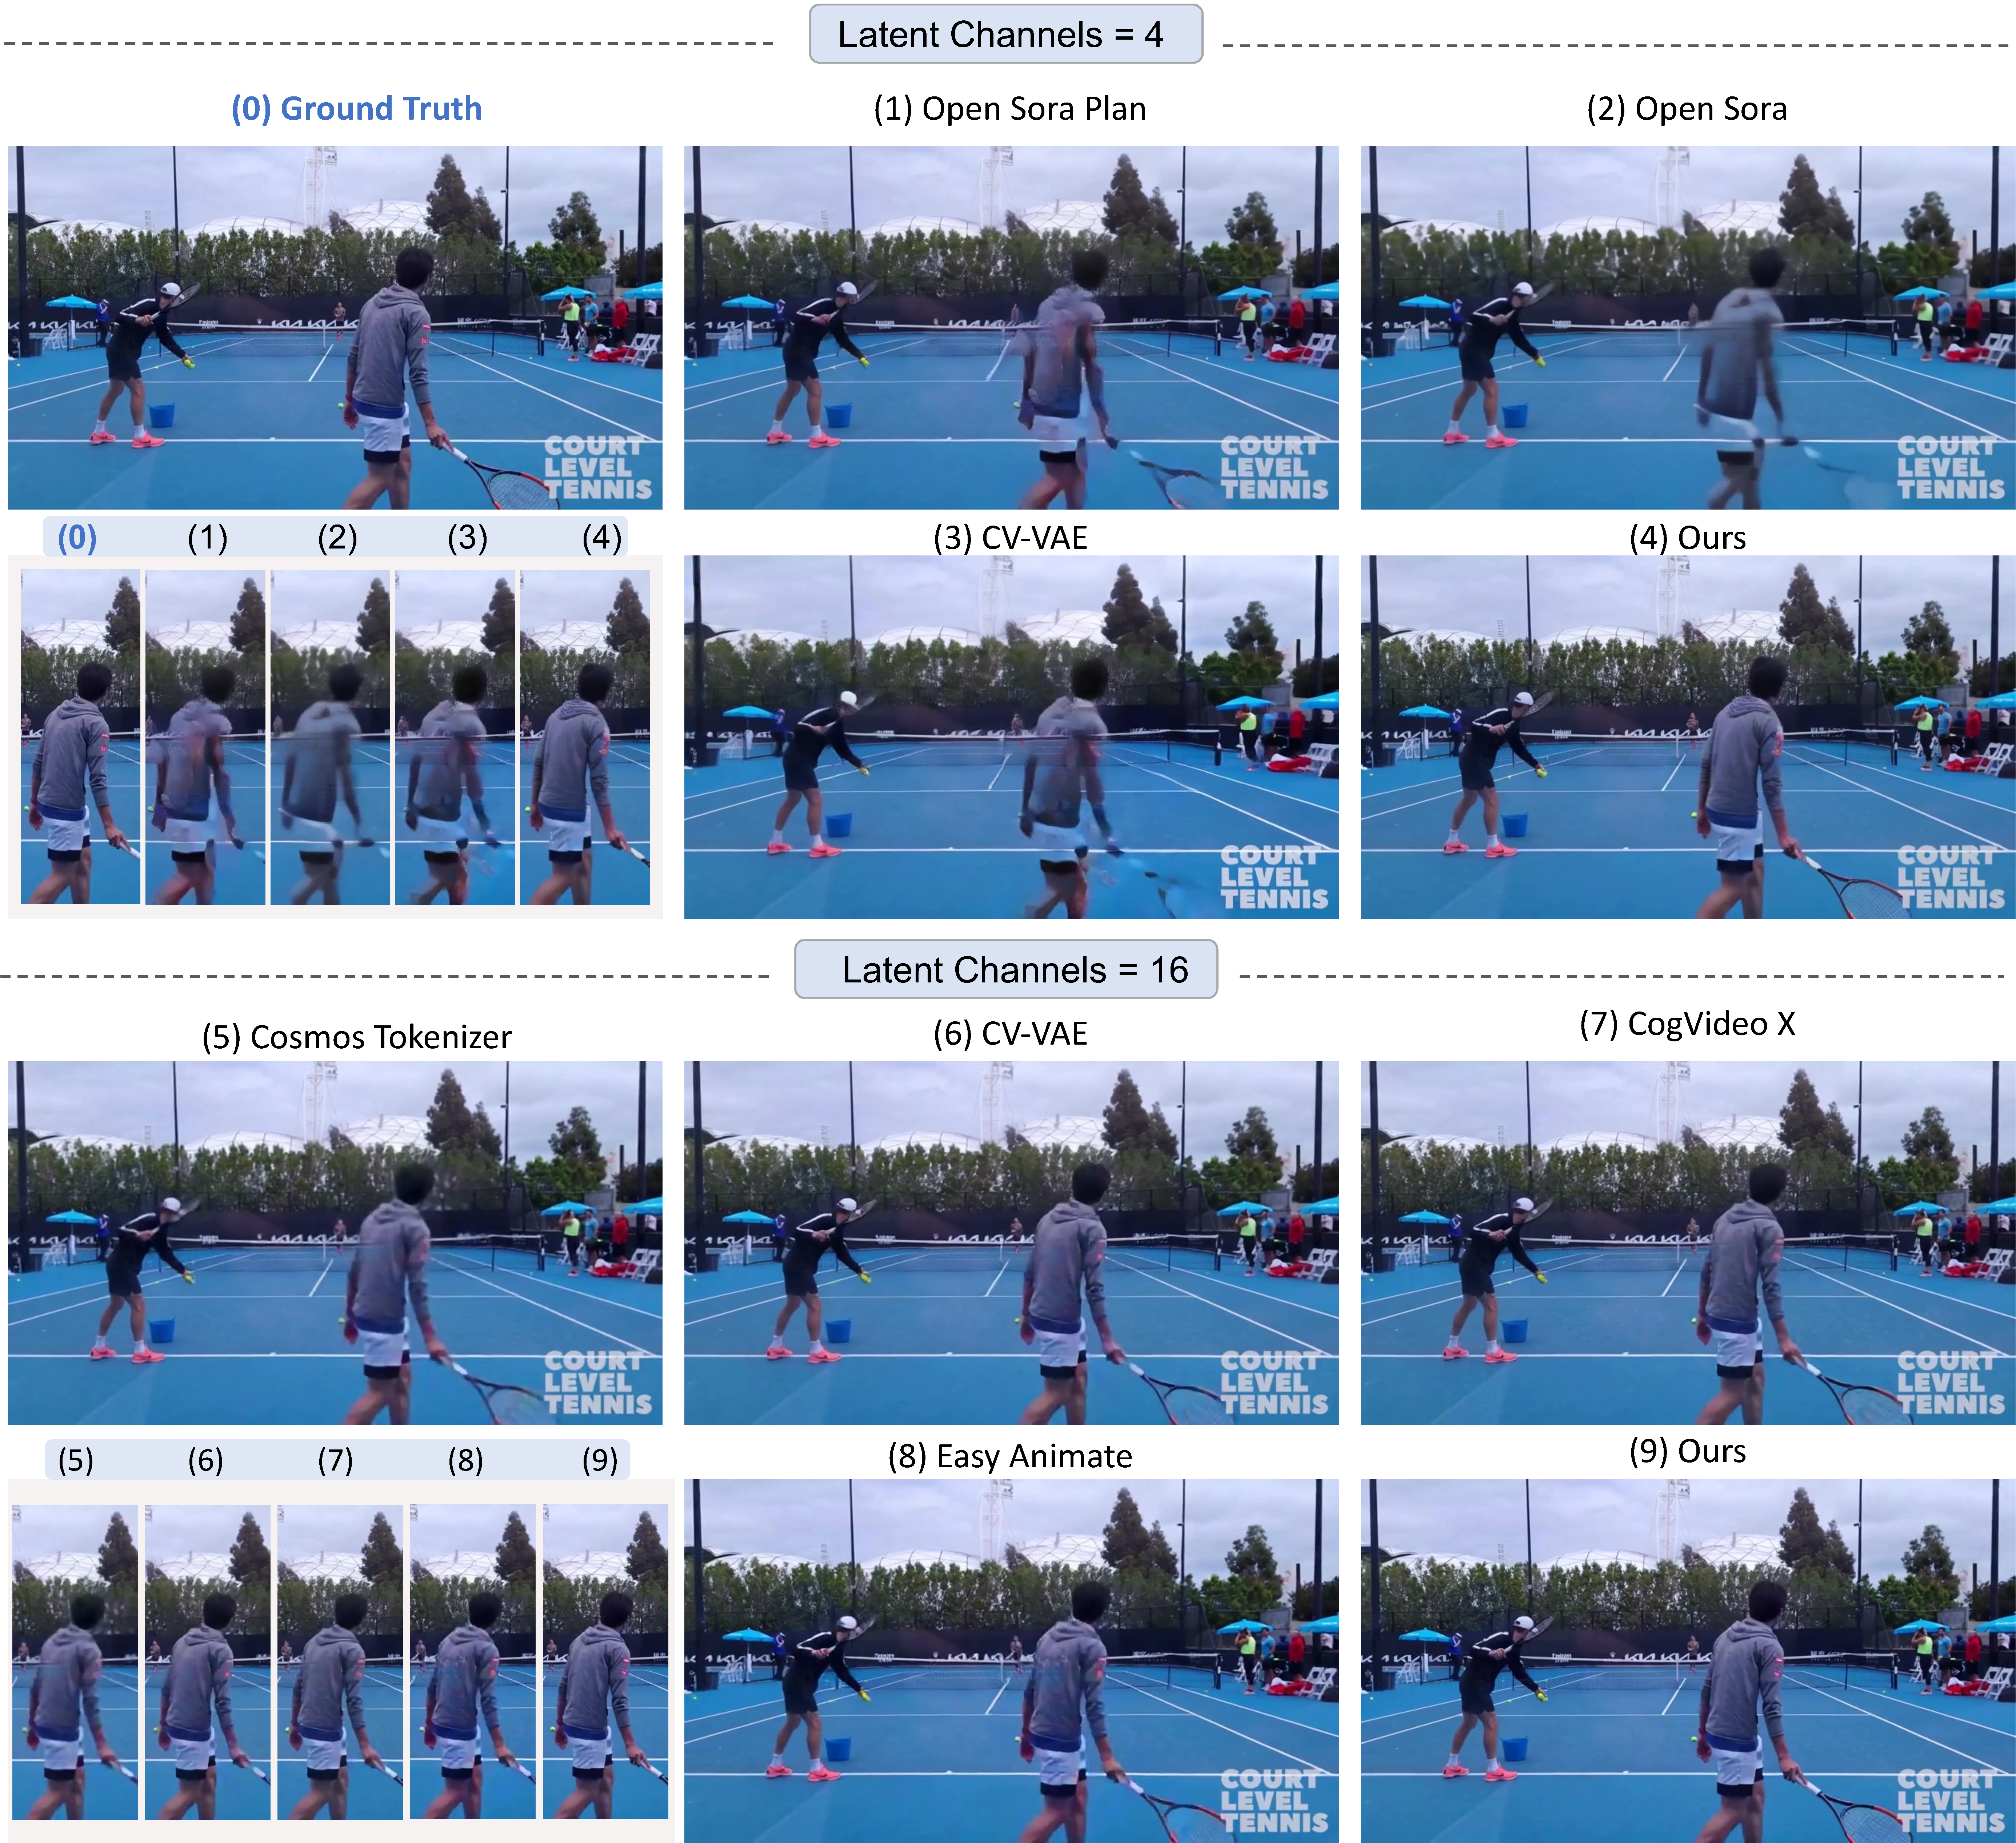
\includegraphics[width=1.0\textwidth]{images/fig1-4and16.pdf}
\caption{
Our reconstruction results compared with a line of three recent strong baseline approaches. 
The ground truth frame is (0). Our model significantly outperforms previous methods, especially under large motion scenarios such as people doing sports.
}
\label{fig:teaser}
\vspace{-3mm}
\end{figure*}



Given the significant attention in the field of video generation, Latent Video Diffusion Models (LVDMs)~\cite{blattmann2023stable, blattmann2023align, he-lvdm, zhou2022magicvideo, he-videocrafter1} have emerged as a popular framework. They have been successfully applied to powerful text-to-video models such as Sora~\cite{videoworldsimulators2024}, VideoCrafter~\cite{he-videocrafter1, chen2024videocrafter2overcomingdatalimitations}, and CogVideoX~\cite{yang2024cogvideox}.
Different from directly generating video pixels, LVDMs generate latent video representations in a compact latent space. This is achieved by first training a Video VAE to encode videos into this latent space.
%
Thus, Video VAE, as a key and fundamental component of LVDMs, has attracted great attention recently.
%
An effective Video VAE can help to reduce the training costs of video diffusion models while improving the final quality of the generated videos.
%
Initially, a series of studies adopt the image VAE from Stable Diffusion~\cite{rombach2022high} for video generation tasks, including AnimateDiff~\cite{guoanimatediff}, MagicVideo~\cite{zhou2022magicvideo}, VideoCrafter1~\cite{he-videocrafter1}, and VideoCrafter2~\cite{chen2024videocrafter2overcomingdatalimitations}. 
%
However, directly adopting an image VAE and compressing video on a frame-by-frame basis leads to temporal flickering due to the lack of temporal correlation. Additionally, the information redundancy along the temporal dimension is not reduced, leading to low training efficiency for subsequent latent video diffusion models.
%
From the introduction of Sora, which compresses videos both temporally and spatially through a Video VAE, a series of studies have emerged that aim to replicate Sora and train their own Video VAEs, including Open Sora~\cite{opensora}, Open Sora Plan~\cite{pku_yuan_lab_and_tuzhan_ai_etc_2024_10948109}, CV-VAE~\cite{zhao2024cv}, CogVideoX~\cite{yang2024cogvideox}, EasyAnimate~\cite{xu2024easyanimatehighperformancelongvideo}, and Cosmos Tokenizer~\cite{cosmos_token}.
%
However, the performance of the current video VAE suffers from many problems, including motion ghost, low-level temporal flickering, blurring (faces, hands, edges, texts), and motion stuttering (lack of correct temporal transition).
% as shown in Fig.~\ref{fig:teaser}.


In this work, we propose a novel cross-modal Video VAE with better spatial and temporal modeling ability in order to solve the aforementioned challenge problems and obtain a robust and high-quality Video VAE.
%
First, we examine different designs for spatial and temporal compression, including simultaneous spatial-temporal (ST) compression and sequential ST compression. 
%
We observed that simultaneous ST compression achieves better low-level temporal smoothness and texture stability, while sequential ST compression achieves better motion recovery, particularly in scenarios of large motion.
%
Thus, we propose a novel architecture that integrates the advantages of both methods and enables effective video detail and motion reconstruction.

Second, we observed that the normally used datasets for text-to-video generation contain text-video pairs. 
Also, during decoding, a text description exists as it serves as the input in the first stage, \textit{i.e.}, the video latent generation stage.
%
To this end, we integrate the text information into the encoding and decoding procedure and propose the first Cross-modal Video VAE.
%
We carefully study how text guidance can be integrated into the spatiotemporal backbone and the mechanism of spatial and temporal semantic guidance. 

In addition, our cross-modal video VAE supports image-video joint training.
To achieve this, we design our network with a fully spatiotemporal factorized architecture, and we feed image and video batches alternately to the network. 
%
During image batches, the data only forwards the spatial part of the network, with the temporal modules being skipped. During video batches, the video forwards both spatial and temporal modules. We also demonstrate that image joint training is crucial for training a video VAE.
%
In summary, our contributions are as follows:
\begin{itemize}
    \item We propose an effective and robust Video VAE, conduct extensive experiments, and achieve the state-of-the-art.
    \item We propose an optimal spatiotemporal modeling approach for Video VAE.
    \item We propose the first cross-modal video VAE that leverages the information from other modalities, i.e., text descriptions, to the best of our knowledge.
    \item Our video VAE is designed and trained to be versatile to conduct both image and video compression. 
\end{itemize}


\section{Related Work}
\subsection{Diffusion Model}
%
In the realm of generative models, diffusion models \cite{ho2020denoising, sohl2015deep} have become foundational due to their exceptional ability to produce high-quality and diverse outputs. Initially developed with the U-Net architecture, these models have demonstrated impressive performance in image and video generation \cite{ramesh2022hierarchical, rombach2022high, ho2022video, saharia2022photorealistic, wei2024dreamvideo, wei2024dreamvideo2, wang2023modelscope, chen2023videocrafter1, chen2024videocrafter2}. 
%

However, the scalability of U-Net-based diffusion models is inherently constrained, posing challenges for applications requiring larger model capacities for enhanced performance. To address this limitation, Diffusion transformers (DiT) \cite{peebles2023scalable} represent a significant advancement. By utilizing the scalable architecture of transformers \cite{vaswani2017attention}, DiT provides an effective means to increase model capacity.
%
A notable achievement in this field is the advancement in generating long videos through the large-scale training of Sora \cite{Sora}, which employs a transformer-based Diffusion architecture for comprehensive simulations of the physical world. This underscores the considerable impact of scaling transformer-based Diffusion models.
%
An increasing number of studies have adopted the Diffusion transformer as the noise estimation network~\cite{chen2023pixart, chen2024pixart, Open-Sora, Open-Sora-Plan, ma2024latte, yang2024cogvideox}.

\subsection{Diffusion Model Acceleration}
%
Despite the notable performance of Diffusion models in image and video synthesis, their significant inference costs hinder practical applications. Efforts to accelerate Diffusion model inference fall into two primary categories. First, techniques such as DDIM~\cite{song2020denoising} allow for fewer sampling steps without sacrificing quality. Additional research has focused on efficient ODE or SDE solvers~\cite{song2019generative, jolicoeur2021gotta, lu2022dpm, karras2022elucidating, lu2022dpm++}, using pseudo numerical methods for faster sampling. Second, approaches include distillation~\cite{salimans2022progressive, wang2023videolcm}, quantization~\cite{li2024q, he2024ptqd, so2024temporal, shang2023post}, and distributed inference~\cite{li2024distrifusion} are employed to reduce the workload and inference time.  

However, these methods often demand additional resources for fine-tuning or optimization. Some training-free approaches~\cite{bolya2023token, wang2024attention} streamline the sampling process by reducing input tokens, thereby eliminating redundancy in image synthesis. Other methods reuse intermediate features between successive timesteps to avoid redundant computations~\cite{wimbauer2024cache, so2023frdiff, zhang2024cross}. DeepCache~\cite{xu2018deepcache} and Faster Diffusion~\cite{li2023faster} utilize feature caching to modify the UNet Diffusion, thus enhancing acceleration. FORA~\cite{selvaraju2024fora} and $\triangle$-DiT~\cite{chen2024delta} adapts this mechanism to DiT by caching residuals between attention layers. PAB~\cite{zhao2024real} caches and broadcasts intermediate features at various timestep intervals based on different attention block characteristics for video synthesis. While these methods have improved Diffusion efficiency, enhancements for DiT in visual synthesis remain limited.
\section{Method}
\label{sec:method}

\subsection{Practical choice of diffusion paradigm}
\label{subsec:practical_dwm}

Building on the background provided in Section \ref{sec:framework}, we now introduce \textsc{diamond} as a practical realization of a diffusion-based world model. In particular, we now define the drift and diffusion coefficients $\mathbf{f}$ and $g$ introduced in Section \ref{subsec:diffusion}, corresponding to a particular choice of diffusion paradigm. While \textsc{ddpm} \citep{ho2020DDPM} is an example of one such choice (as described in Appendix \ref{app:ddpm}) and would historically be the natural candidate, we instead build upon the \textsc{edm} formulation proposed in \citet{karras2022elucidating}. The practical implications of this choice are discussed in Section \ref{subsec:diffusion_choice}. In what follows, we describe how we adapt \textsc{edm} to build our diffusion-based world model.

We consider the perturbation kernel $p^{0\tau}(\x_{t+1}^\tau \mid \x_{t+1}^0) = \mathcal{N}(\x_{t+1}^\tau; \x_{t+1}^0, \sigma^2(\tau) \mathbf{I})$, where $\sigma(\tau)$ is a real-valued function of diffusion time called the noise schedule. This corresponds to setting the drift and diffusion coefficients to $\mathbf{f}(\x, \tau) = \mathbf{0}$ (affine) and $g(\tau) = \sqrt{2 \dot \sigma(\tau) \sigma(\tau)}$.

We use the network preconditioning introduced by \citet{karras2022elucidating} and so parameterize $\mathbf{D}_\theta$ in Equation \ref{eq:denoising_sm_conditional} as the weighted sum of the noised observation and the prediction of a neural network $\mathbf{F}_\theta$,
\begin{equation}
\label{eq:karras_wrappers} 
    \mathbf{D}_\theta(\x_{t+1}^\tau, y_t^\tau) = c_\text{skip}^\tau \; \x_{t+1}^\tau + c_\text{out}^\tau \; \mathbf{F}_\theta \big( c_\text{in}^\tau \; \x_{t+1}^\tau, y_t^\tau \big),
\end{equation}
where for brevity we define $y_t^\tau \coloneqq (c_\text{noise}^\tau, \x^0_{\le t}, a_{\le t})$ to include all conditioning variables.

The preconditioners $c_\text{in}^\tau$ and $c_\text{out}^\tau$ are selected to keep the network's input and output at unit variance for any noise level $\sigma(\tau)$, $c_\text{noise}^\tau$ is an empirical transformation of the noise level, and $c_\text{skip}^\tau$ is given in terms of $\sigma(\tau)$ and the standard deviation of the data distribution $\sigma_\text{data}$, as $c_{skip}^\tau = \sigma_{data}^2/(\sigma_{data}^2 + \sigma^2(\tau))$. These preconditioners are fully described in Appendix \ref{appendix:karras_conditioners}.

Combining Equations \ref{eq:denoising_sm_conditional} and \ref{eq:karras_wrappers} provides insight into the training objective of $\mathbf{F}_\theta$,
\begin{align}
\label{eq:effective_obj}
\mathcal{L}(\theta)  = \bbe \Big[ \Vert 
\underbrace{\mathbf{F}_\theta \big( c_\text{in}^\tau \x_{t+1}^\tau, y_t^\tau \big)}_\text{Network prediction} - 
\underbrace{\frac{1}{c_\text{out}^\tau} \big( \x_{t+1}^0 - c_\text{skip}^\tau \x_{t+1}^\tau\big)}_\text{Network training target}
\Vert^2 \Big].
\end{align}
The network training target adaptively mixes signal and noise depending on the degradation level $\sigma(\tau)$.
When $\sigma(\tau) \gg \sigma_\text{data}$, we have $c_\text{skip}^\tau \to 0$, and the training target for $\mathbf{F}_\theta$ is dominated by the clean signal $\x_{t+1}^0$. Conversely, when the noise level is low, $\sigma(\tau) \to 0$, we have $c_\text{skip}^\tau \to 1$, and the target becomes the difference between the clean and the perturbed signal, i.e. the added Gaussian noise. Intuitively, this prevents the training objective to become trivial in the low-noise regime. In practice, this objective is high variance at the extremes of the noise schedule, so \citet{karras2022elucidating} sample the noise level $\sigma(\tau)$ from an empirically chosen log-normal distribution in order to concentrate the training around medium-noise regions, as described in Appendix \ref{appendix:karras_conditioners}.

We use a standard U-Net 2D for the vector field $\mathbf{F}_\theta$ \citep{ronneberger2015unet}, and we keep a buffer of $L$ past observations and actions that we use to condition the model. We concatenate these past observations to the next noisy observation channel-wise, and we input actions through adaptive group normalization layers \citep{adagn} in the residual blocks \citep{He2015} of the U-Net.

As discussed in Section \ref{subsec:dwm_training} and Appendix \ref{appendix:sampling}, there are many possible sampling methods to generate the next observation from the trained diffusion model. While our codebase supports a variety of sampling schemes, we found Euler's method to be effective without incurring the cost of additional NFE required by higher order samplers, or the unnecessary complexity of stochastic sampling.

\subsection{Reinforcement learning in imagination}
\label{subsec:rl}

Given the diffusion model from Section \ref{subsec:practical_dwm}, we now complete our world model with a reward and termination model, required for training an RL agent in imagination. Since estimating the reward and termination are scalar prediction problems, we use a separate model $R_\psi$ consisting of standard \textsc{cnn} \citep{cnn_lecun,He2015} and \textsc{lstm} \citep{lstm,Gers2000} layers to handle partial observability. The RL agent involves an actor-critic network parameterized by a shared \textsc{cnn-lstm} with policy and value heads. The policy $\pi_\phi$ is trained with \textsc{reinforce} with a value baseline, and we use a Bellman error with $\lambda$-returns to train the value network $V_\phi$, similar to \citet{iris2023}. We train the agent entirely in imagination as described in Section \ref{subsec:pomdp_and_wm}. The agent only interacts with the real environment for data collection. After each collection stage, the current world model is updated by training on all data collected so far. Then, the agent is trained with RL in the updated world model environment, and these steps are repeated. This procedure is detailed in Algorithm \ref{alg:diamond}, and is similar to \citet{kaiser2019atari100k,hafner2020dream,iris2023}. We provide architecture details, hyperparameters, and RL objectives in Appendices \ref{app:architectures}, \ref{app:hyperparams}, \ref{appendix:rl_actor_critic}, respectively.

\section{Experiments}
\label{sec:exp}

\begin{table}[t]
\small\centering\setlength{\tabcolsep}{3pt}
\begin{tabular}{l | c | g | g g g g }
\toprule
\rowcolor{white} \textbf{ImageNet 256$\times$256} & Latent Shape & Autoencoder & rFID $\downarrow$ & PSNR $\uparrow$ & SSIM $\uparrow$ & LPIPS $\downarrow$ \\
\midrule
\rowcolor{white} \multirow{2}{*}{f32c32} & \multirow{2}{*}{8$\times$8$\times$32} 
 & SD-VAE \tablecite{rombach2022high} & 2.64 & 22.13 & 0.59 & 0.117 \\
 & & \modelshort                      & \textbf{0.69} & \textbf{23.85} & \textbf{0.66} & \textbf{0.082} \\
\midrule
\rowcolor{white} \multirow{2}{*}{f64c128} & \multirow{2}{*}{4$\times$4$\times$128}
 & SD-VAE \tablecite{rombach2022high} & 26.65 & 18.07 & 0.41 & 0.283 \\
 & & \modelshort                      & \textbf{0.81} & \textbf{23.60} & \textbf{0.65} & \textbf{0.087} \\
\bottomrule
\toprule
\rowcolor{white} \textbf{ImageNet 512$\times$512} & Latent Shape & Autoencoder & rFID $\downarrow$ & PSNR $\uparrow$ & SSIM $\uparrow$ & LPIPS $\downarrow$ \\
 \midrule
\rowcolor{white} \multirow{2}{*}{f64c128} & \multirow{2}{*}{8$\times$8$\times$128}
 & SD-VAE \tablecite{rombach2022high} & 16.84 & 19.49 & 0.48 & 0.282 \\
 & & \modelshort                      & \textbf{0.22} & \textbf{26.15} & \textbf{0.71} & \textbf{0.080} \\
\midrule
\rowcolor{white} \multirow{2}{*}{f128c512} & \multirow{2}{*}{4$\times$4$\times$512}
 & SD-VAE \tablecite{rombach2022high} & 100.74 & 15.90 & 0.40 & 0.531 \\
 & & \modelshort                      & \textbf{0.23} & \textbf{25.73} & \textbf{0.70} & \textbf{0.084} \\
\bottomrule
\toprule
\rowcolor{white} \textbf{FFHQ 1024$\times$1024} & Latent Shape & Autoencoder & rFID $\downarrow$ & PSNR $\uparrow$ & SSIM $\uparrow$ & LPIPS $\downarrow$ \\
\midrule
\rowcolor{white} \multirow{2}{*}{f64c128} & \multirow{2}{*}{16$\times$16$\times$128}
 & SD-VAE \tablecite{rombach2022high} & 6.62 & 24.55 & 0.68 & 0.237 \\
 & & \modelshort                      & \textbf{0.23} & \textbf{31.04} & \textbf{0.83} & \textbf{0.061} \\
 \midrule
\rowcolor{white} \multirow{2}{*}{f128c512} & \multirow{2}{*}{8$\times$8$\times$512}
 & SD-VAE \tablecite{rombach2022high} & 179.71 & 18.11 & 0.63 & 0.585 \\
 & & \modelshort                      &  \textbf{0.41} & \textbf{31.18} & \textbf{0.83} & \textbf{0.062} \\
\bottomrule
\toprule
\rowcolor{white} \textbf{MapillaryVistas 2048$\times$2048} & Latent Shape & Autoencoder & rFID $\downarrow$ & PSNR $\uparrow$ & SSIM $\uparrow$ & LPIPS $\downarrow$ \\ 
 \midrule
\rowcolor{white} \multirow{2}{*}{f64c128} & \multirow{2}{*}{32$\times$32$\times$128}
 & SD-VAE \tablecite{rombach2022high} & 7.55 & 22.37 & 0.68 & 0.262 \\
 & & \modelshort                      & \textbf{0.36} & \textbf{29.57} & \textbf{0.84} & \textbf{0.075} \\
 \midrule
\rowcolor{white} \multirow{2}{*}{f128c512} & \multirow{2}{*}{16$\times$16$\times$512} 
 & SD-VAE \tablecite{rombach2022high} & 152.09 & 17.82 & 0.67 & 0.594 \\
 & & \modelshort                      &  \textbf{0.38} & \textbf{29.70} & \textbf{0.84} & \textbf{0.074} \\
\bottomrule
\end{tabular}
\vspace{-5pt}
\caption{\textbf{Image Reconstruction Results.}}
\vspace{-10pt}
\label{tab:ae_main}
\end{table}

\subsection{Setups}

\paragraph{Implementation Details.} We use a mixture of datasets to train autoencoders (baselines and \modelshort), containing ImageNet \citep{deng2009imagenet}, SAM \citep{kirillov2023segment}, MapillaryVistas \citep{neuhold2017mapillary}, and FFHQ \citep{karras2019style}. For ImageNet experiments, we exclusively use the ImageNet training split to train autoencoders and diffusion models. The model architecture is similar to SD-VAE \citep{rombach2022high} except for our new designs discussed in Section~\ref{sec:main_model}. In addition, we use the original autoencoders instead of the variational autoencoders for our models, as they perform the same in our experiments and the original autoencoders are simpler. We also replace transformer blocks with EfficientViT blocks \citep{cai2023efficientvit} to make autoencoders more friendly for handling high-resolution images while maintaining similar accuracy. 

For image generation experiments, we apply autoencoders to diffusion transformer models including DiT \citep{peebles2023scalable} and UViT \citep{bao2023all}. We follow the same training settings as the original papers. 
We consider three settings with different resolutions, including ImageNet \citep{deng2009imagenet} for $512 \times 512$ generation, FFHQ \citep{karras2019style} and MJHQ \citep{li2024playground} for $1024 \times 1024$ generation, and MapillaryVistas \citep{neuhold2017mapillary} for $2048 \times 2048$ generation. 

\begin{table}[t]
\small\centering\setlength{\tabcolsep}{2pt}
\begin{tabular}{l | g | g | g g | g | g | g g }
\toprule
\rowcolor{white} Diffusion & & Patch & \multicolumn{2}{c|}{Throughput (image/s) $\uparrow$} & Latency & Memory & \multicolumn{2}{c}{FID $\downarrow$} \\
\rowcolor{white} Model & \multirow{-2}{*}{Autoencoder} & Size & Training & Inference & (ms) $\downarrow$ & (GB) $\downarrow$ & w/o CFG & w/ CFG \\
\midrule
\rowcolor{white} & SD3-VAE-f8 \tablecite{esser2024scaling}                   & 2 &  352 &  2984 & 3.8 & 13.8 & 164.34 & 143.82 \\
\rowcolor{white} & Flux-VAE-f8 \tablecite{flux2024}                          & 2 &  352 &  2984 & 3.8 & 13.8 & 106.07 & 84.73 \\
\cmidrule{2-9}
\rowcolor{white} & SDXL-VAE-f8 \tablecite{podell2023sdxl}                    & 2 &  352 &  2991 & 3.8 & 13.8 & 51.03 & 26.38 \\
\rowcolor{white} & Asym-VAE-f8 \tablecite{zhu2023designing}                  & 2 &  352 &  2991 & 3.8 & 13.8 & 51.96 & 24.57 \\
\rowcolor{white} & SD-VAE-f8 \tablecite{rombach2022high}                     & 2 &  352 &  2991 & 3.8 & 13.8 & 51.96 & 24.57 \\
\rowcolor{white} & SD-VAE-f16 \tablecite{rombach2022high}                    & 2 & 1550 & 12881 & 1.3 &  4.0 & 76.86 & 44.22 \\
\rowcolor{white} & SD-VAE-f32 \tablecite{rombach2022high}                    & 1 & 1551 & 12883 & 1.3 &  4.0 & 70.23 & 38.63 \\
\cmidrule{2-9}
& \modelshort-f32                                                            & 1 & 1553 & 12850 & 1.3 &  4.0 & \textbf{46.12} & \textbf{18.08} \\ 
& \modelshort-f64                                                            & 1 & \textbf{6295} & \textbf{53774} & \textbf{0.7} & \textbf{1.5} & 67.30 & 35.96 \\
\multirow{-11}{*}{UViT-S \tablecite{bao2023all}} & \:\:\modelshort-f64$^\dag$ & 1 & \textbf{6295} & \textbf{53774} & \textbf{0.7} & \textbf{1.5} & 61.84 & 30.63 \\
\midrule
\midrule
\rowcolor{white} & Flux-VAE-f8 \tablecite{flux2024}                          & 2 &   54 &  416 & 31.7 & 56.3 & 27.35 & 8.72 \\
\cmidrule{2-9}
\rowcolor{white} & Asym-VAE-f8 \tablecite{zhu2023designing}                  & 2 &   54 &  424 & 31.7 & 56.2 & 11.55 & 2.95 \\
\rowcolor{white} &  SD-VAE-f8 \tablecite{rombach2022high}                    & 2 &   54 &  424 & 31.7 & 56.2 & 12.03 & 3.04 \\
\cmidrule{2-9}
& \modelshort-f32                                                            & 1 &  \textbf{241} &  \textbf{2016} & \textbf{7.8} & \textbf{20.9} &  9.56 & 2.84 \\
\multirow{-5}{*}{DiT-XL \tablecite{peebles2023scalable}} 
& \:\:\modelshort-f32$^\ddag$                                                    & 1 &  \textbf{241} &  \textbf{2016} & \textbf{7.8} & \textbf{20.9} &  \textbf{6.88} & \textbf{2.41} \\


\midrule
\midrule
\rowcolor{white} & Flux-VAE-f8 \tablecite{flux2024}                          & 2 &  55 &  349 & 30.4 & 54.2 & 30.91 & 12.63 \\
\cmidrule{2-9}
\rowcolor{white} & Asym-VAE-f8 \tablecite{zhu2023designing}                  & 2 &  55 &  351 & 30.3 & 54.1 & 11.36 &  3.51 \\
\rowcolor{white}  & SD-VAE-f8 \tablecite{rombach2022high}                    & 2 &   \,\,55\,\,\tikzmark{uvit_h_f8p2:a1} &   \,\,351\,\,\tikzmark{uvit_h_f8p2:a2} & 30.3 & 54.1 & 11.04 & \,\,3.55\,\,\tikzmark{uvit_h_f8p2:a3} \\
\cmidrule{2-9}
& \modelshort-f32                                                            & 1 &  247 &  1622 &  8.2 & 18.6 &  \textbf{9.83} & \textbf{2.53} \\
& \modelshort-f64                                                            & 1 & \,\,\textbf{984}\,\,\tikzmark{uvit_h_f64p1:a1} &  \,\,\textbf{6706}\,\,\tikzmark{uvit_h_f64p1:a2} & \textbf{3.5} & \textbf{10.6} & 13.96 & \,\,3.01\,\,\tikzmark{uvit_h_f64p1:a3} \\
\multirow{-6}{*}{UViT-H \tablecite{bao2023all}} & \:\:\modelshort-f64$^\dag$ & 1 & \textbf{984} &  \textbf{6706} & \textbf{3.5} & \textbf{10.6} & 12.26 & 2.66 \\

\midrule
\midrule
\rowcolor{white} & Asym-VAE-f8 \tablecite{zhu2023designing}                   & 2 &  27 & 157 & 74.8 & OOM & 9.87 & 3.62 \\
\rowcolor{white}  & SD-VAE-f8 \tablecite{rombach2022high}                     & 2 &  27 & 157 & 74.8 & OOM & 9.73 & 3.57 \\
\cmidrule{2-9}
& \modelshort-f32                                                             & 1 & 112 & 665 & 19.7 & 42.0 & 8.13 & 2.30 \\
& \modelshort-f64                                                             & 1 & \textbf{450} & \textbf{2733} & \textbf{8.6} & \textbf{30.2} & 7.78 & 2.47 \\
\multirow{-5}{*}{UViT-2B \tablecite{bao2023all}} & \:\:\modelshort-f64$^\dag$ & 1 & \textbf{450} & \textbf{2733} & \textbf{8.6} & \textbf{30.2} & \textbf{6.50} & \textbf{2.25} \\

\bottomrule
\end{tabular}

\begin{tikzpicture}[overlay, remember picture, shorten >=.5pt, shorten <=.5pt, transform canvas={yshift=.25\baselineskip}]

\draw [->, red] ({pic cs:uvit_h_f8p2:a1}) [bend left] to node [below right] (uvit_h_f8p2:t1) {\hspace{-2pt}\scriptsize \textbf{17.9$\times$}} ({pic cs:uvit_h_f64p1:a1});

\draw [->, red] ({pic cs:uvit_h_f8p2:a2}) [bend left] to node [below right] (uvit_h_f8p2:t2) {\hspace{-2pt}\scriptsize \textbf{19.1$\times$}} ({pic cs:uvit_h_f64p1:a2});

\draw [->, red] ({pic cs:uvit_h_f8p2:a3}) [bend left] to node [below right] (uvit_h_f8p2:t3) {\hspace{-2pt}\scriptsize \textbf{-0.54}} ({pic cs:uvit_h_f64p1:a3});

\end{tikzpicture}
\vspace{-5pt}
\caption{\textbf{Class-Conditional Image Generation Results on ImageNet 512$\times$512.} $^\dag$ represents the model is trained for 4$\times$ training iterations (i.e., 500K $\rightarrow$ 2,000K iterations). $^\ddag$ represents the model is trained with 4$\times$ batch size (i.e., 256 $\rightarrow$ 1024).}
\label{tab:diffusion_imagenet_main}
\end{table}


\begin{table}[t]
\small\centering\setlength{\tabcolsep}{2pt}
\begin{tabular}{l | g | g | g g | g | g | g g }
\toprule
\rowcolor{white} Diffusion & & Patch & \multicolumn{2}{c|}{Throughput (image/s) $\uparrow$} & Latency & Memory & \multicolumn{2}{c}{MJHQ 512$\times$512} \\
\rowcolor{white} Model & \multirow{-2}{*}{Autoencoder} & Size & Training & Inference & (ms) $\downarrow$ & (GB) $\downarrow$ & FID $\downarrow$ & CLIP Score $\uparrow$ \\
\midrule
\rowcolor{white} & SD-VAE-f8 \tablecite{rombach2022high} & 2 & 43 & 312 & 37.1 & 60.45 & 6.3 & 26.36 \\
\multirow{-2}{*}{PIXART-$\alpha$ \tablecite{chenpixart}} 
& \modelshort-f32                                        & 1 & \textbf{173} & \textbf{1251} & \textbf{10.4} & \textbf{23.77} & \textbf{6.1} & \textbf{26.41} \\
\bottomrule
\end{tabular}
\vspace{-5pt}
\caption{\textbf{Text-to-Image Generation Results.}}
\vspace{-10pt}
\label{tab:diffusion_t2i_main}
\end{table}


\begin{figure}[t]
    \centering
    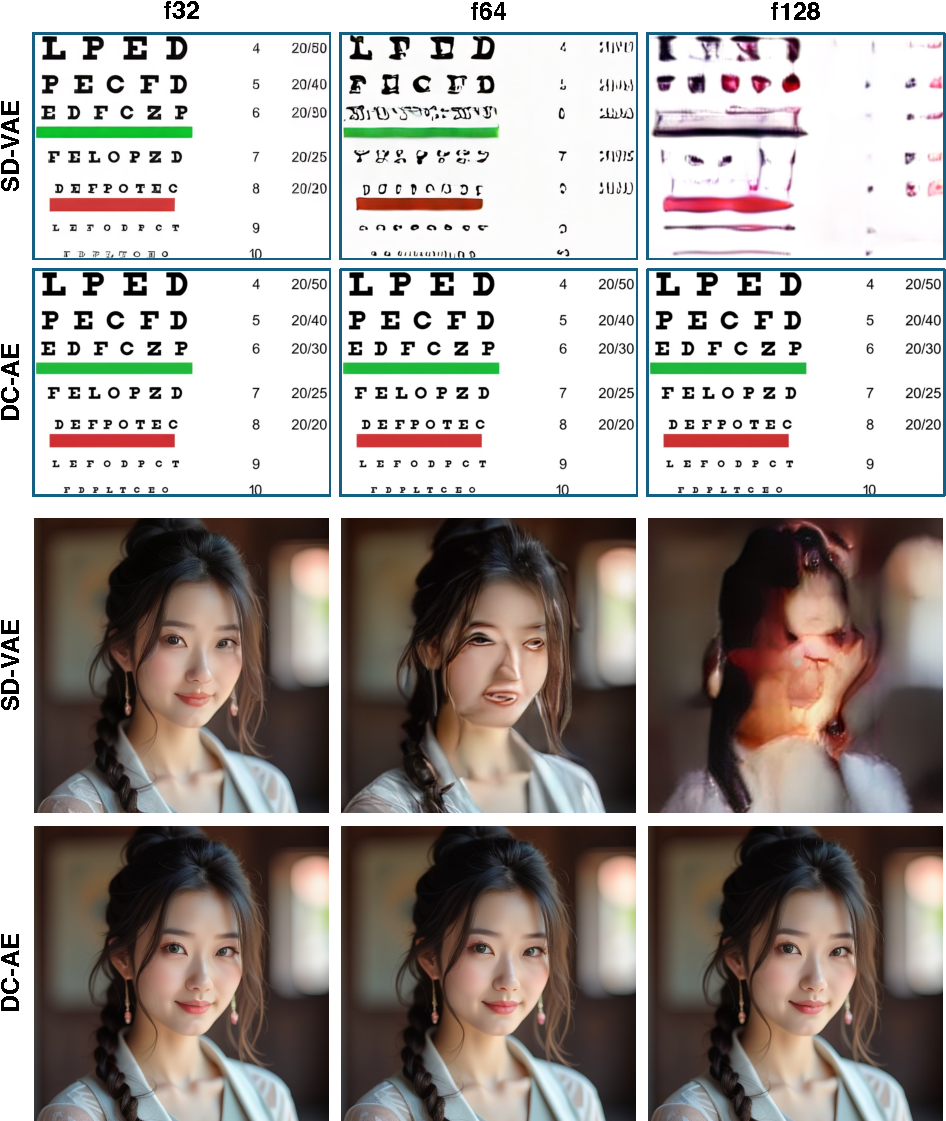
\includegraphics[width=0.95\linewidth]{figures/src/ae_visualization.pdf}
    \vspace{-10pt}
    \caption{\textbf{Autoencoder Image Reconstruction Samples.}}
    \vspace{-10pt}
    \label{fig:ae_visualization}
\end{figure}


\begin{figure}[t]
    \centering
    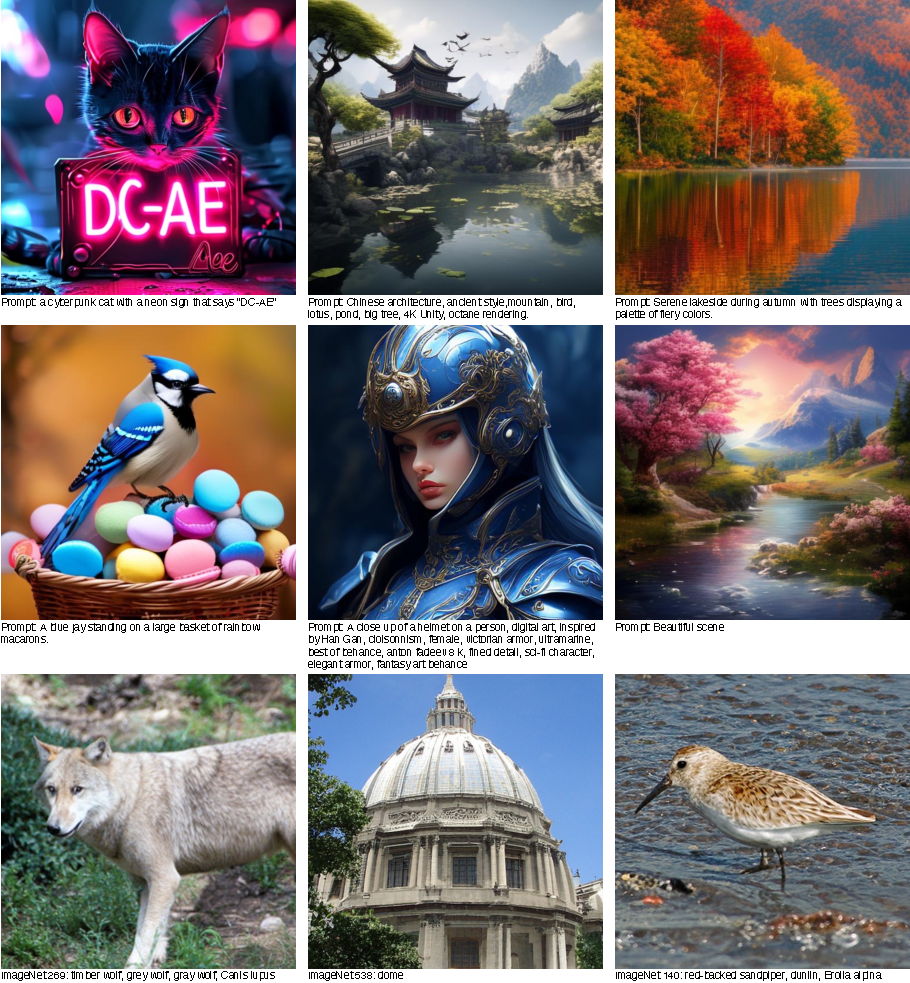
\includegraphics[width=1\linewidth]{figures/src/diffusion_visualization.pdf}
    \vspace{-15pt}
    \caption{\textbf{Images Generated by Diffusion Model using Our \modelshort.}}
    \vspace{-10pt}
    \label{fig:diffusion_visualization}
\end{figure}


\paragraph{Efficiency Profiling.} We profile the training and inference throughput on the H100 GPU with PyTorch and TensorRT respectively. The latency is measured on the 3090 GPU with batch size 2. The training memory is profiled using PyTorch, assuming a batch size of 256. We use fp16 for all cases. For simplicity, we assume the number of sampling steps is 1.

\subsection{Image Compression and Reconstruction}
Table~\ref{tab:ae_main} summarizes the results of \modelshort and SD-VAE \citep{rombach2022high} under various settings (f represents the spatial compression ratio and c denotes the number of latent channels). \modelshort provides significant reconstruction accuracy improvements than SD-VAE for all cases. For example, on ImageNet $512 \times 512$, \modelshort improves the rFID from 16.84 to 0.22 for the f64c128 autoencoder and 100.74 to 0.23 for the f128c512 autoencoder. 

In addition to the quantitative results, Figure~\ref{fig:ae_visualization} shows image reconstruction samples produced by SD-VAE and \modelshort. Reconstructed images by \modelshort demonstrate a better visual quality than SD-VAE's reconstructed images. In particular, for the f64 and f128 autoencoders,  \modelshort still maintains a good visual quality for small text and the human face. 

\subsection{Latent Diffusion Models}
We compare \modelshort with the widely used SD-VAE-f8 autoencoder \citep{rombach2022high} on various diffusion transformer models. For \modelshort, we always use a patch size of 1 (denoted as p1). For SD-VAE-f8, we follow the common setting and use a patch size of 2 or 4 (denoted as p2, p4). The results are summarized in Table~\ref{tab:diffusion_imagenet_main}, Table~\ref{tab:diffusion_hr_main}, and Table~\ref{tab:diffusion_t2i_main}. 

\vspace{-5pt}
\paragraph{ImageNet 512$\times$512.} As shown in Table~\ref{tab:diffusion_imagenet_main}, \modelshort-f32p1 consistently delivers better FID than SD-VAE-f8p2 on all diffusion transformer models. In addition, it has 4$\times$ fewer tokens than SD-VAE-f8p2, leading to 4.5$\times$ higher H100 training throughput and 4.8$\times$ higher H100 inference 
\begin{wrapfigure}{r}{0.35\textwidth}
  \vspace{-10pt}
  \begin{center}
    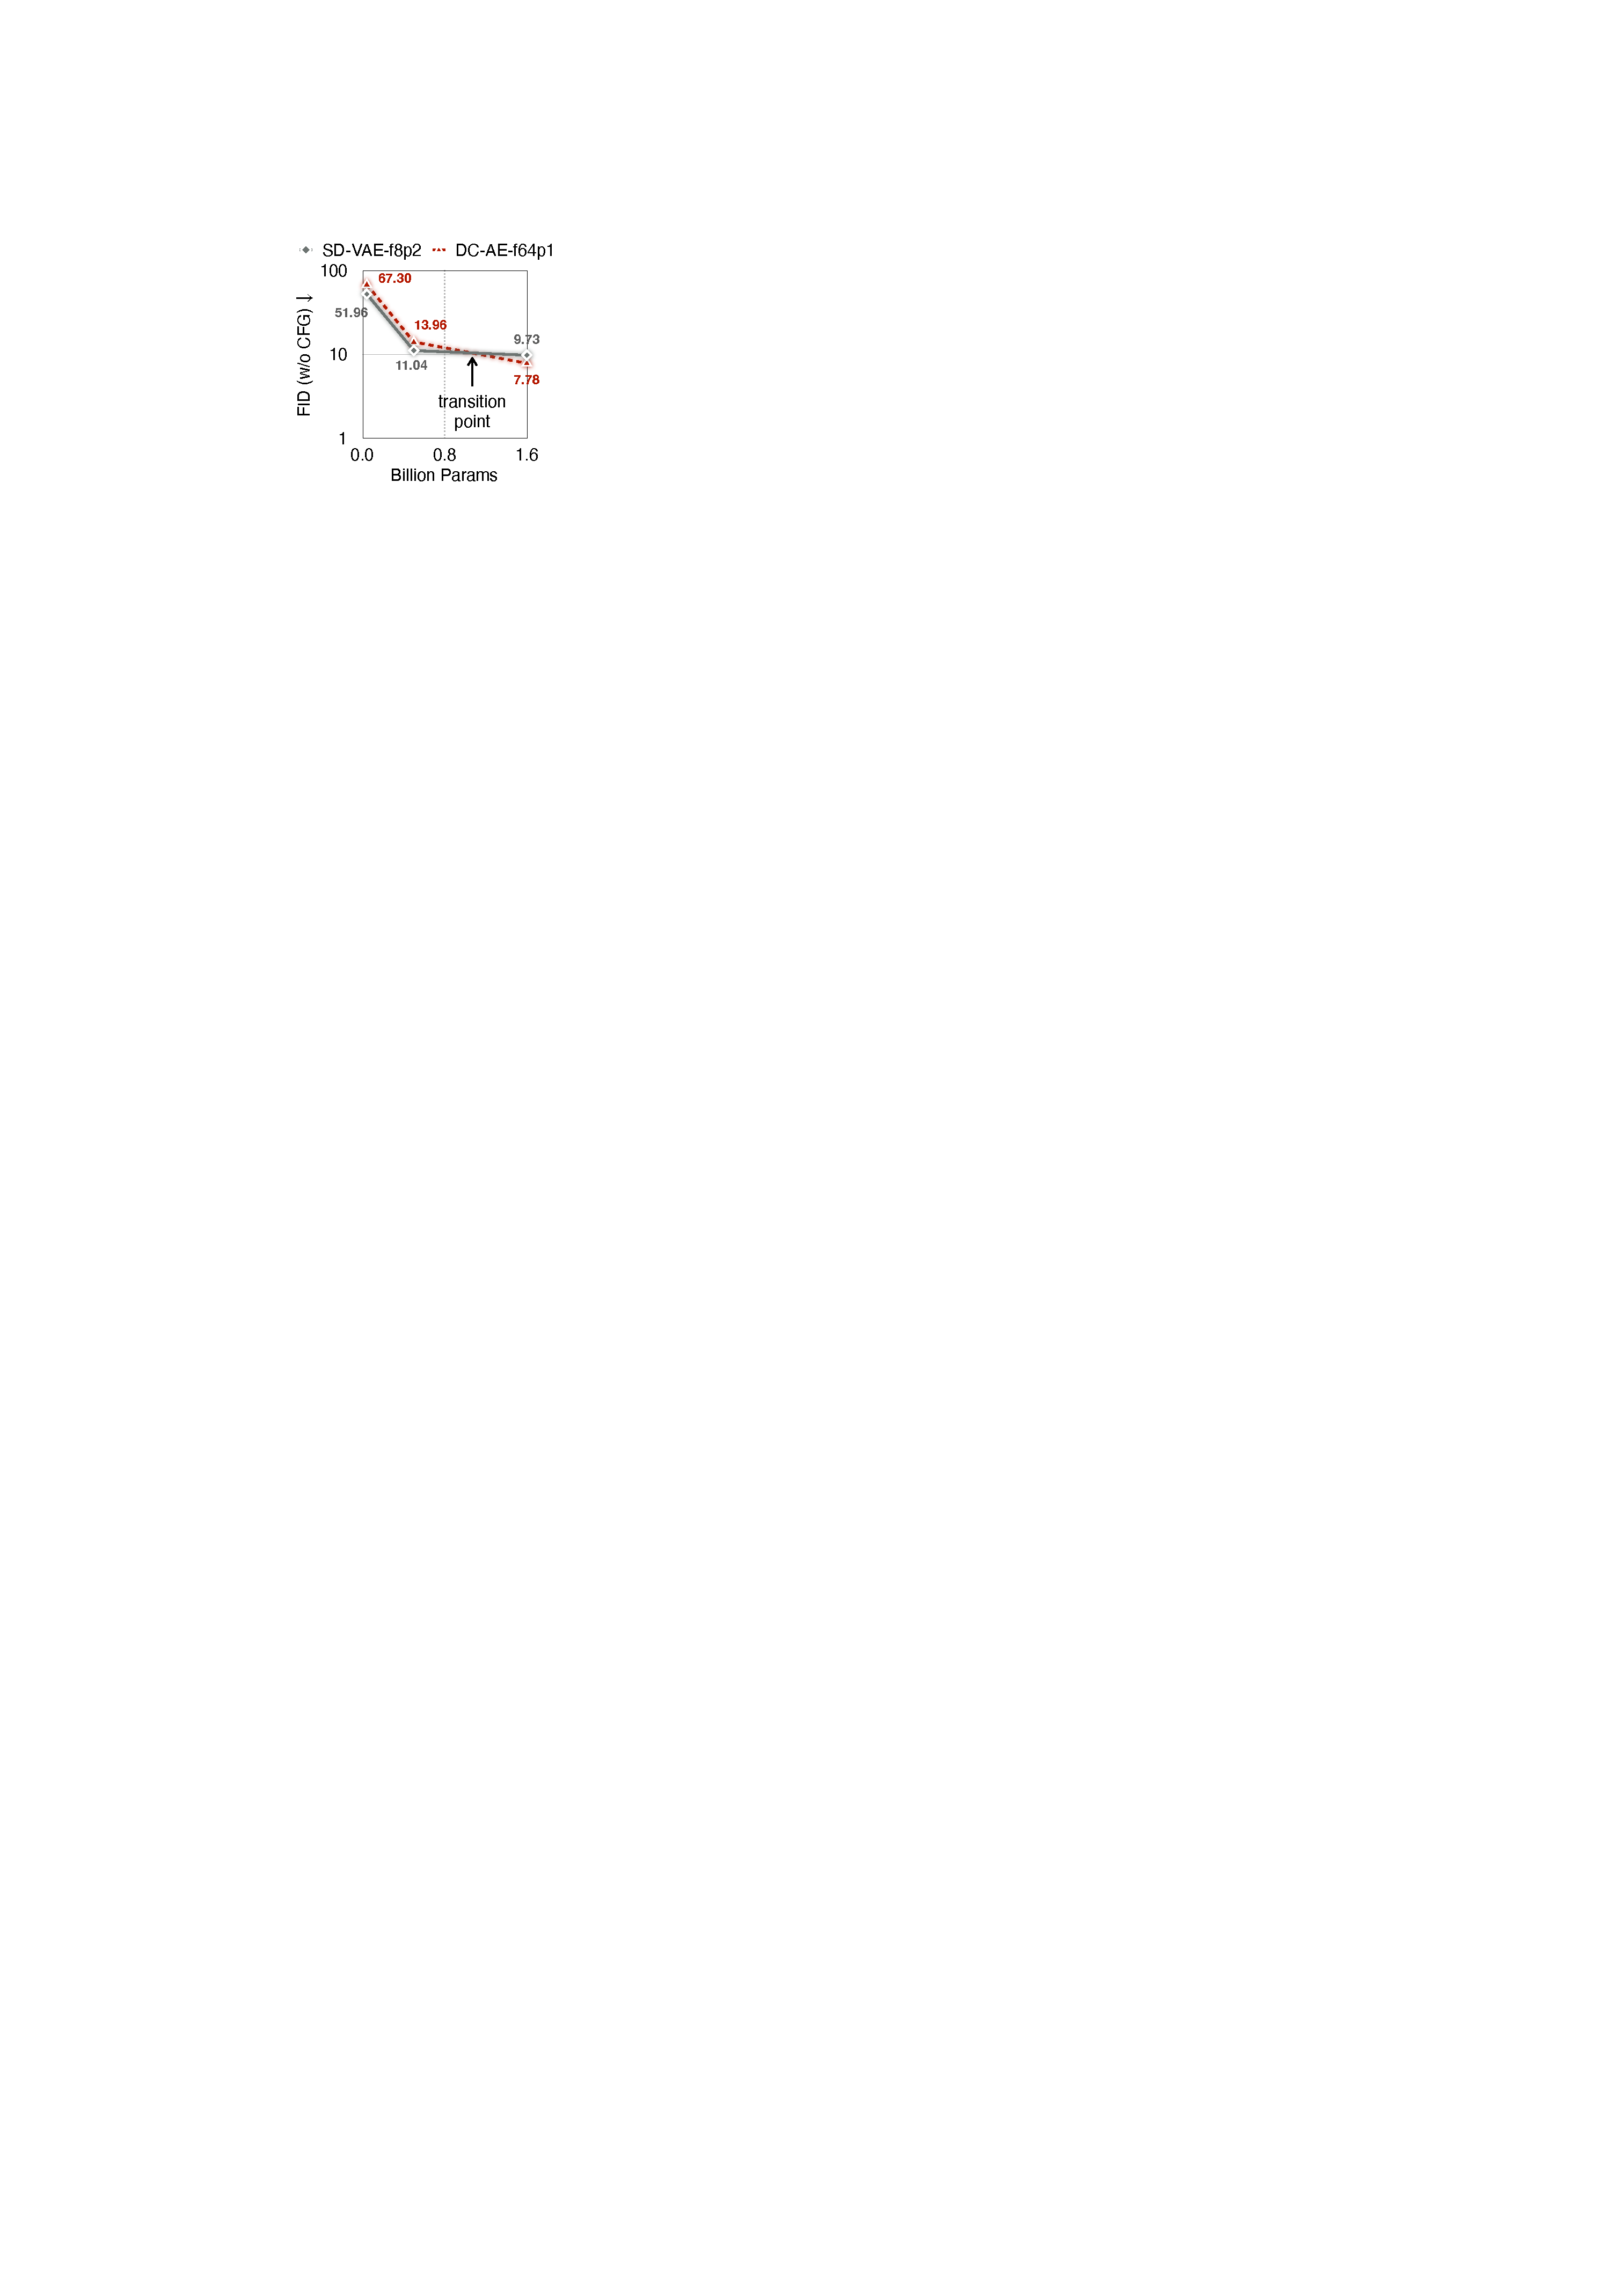
\includegraphics[width=0.35\textwidth]{figures/src/diffusion_scaling_up.pdf}
  \end{center}
  \vspace{-10pt}
  \caption{\textbf{Model Scaling Results on ImageNet 512$\times$512 with UViT.} \modelshort-f64 benefits more from scaling up than SD-VAE-f8.}
  \vspace{-20pt}
  \label{fig:diffusion_scaling_up}
\end{wrapfigure}

\!\!\!\! throughput for DiT-XL. We also observe that larger diffusion transformer models seem to benefit more from our \modelshort. For example, \modelshort-f64p1 has a worse FID than SD-VAE-f8p2 on UViT-S but a better FID on UViT-H. We conjecture it is because \modelshort-f64 has a larger latent channel number than SD-VAE-f8, thus needing more model capacity \citep{esser2024scaling}. 

\vspace{-10pt}
\paragraph{Text-to-Image Generation.} Table~\ref{tab:diffusion_t2i_main} reports our text-to-image generation results. All models are trained for 100K iterations from scratch. Similar to prior cases, we observe \modelshort-f32p1 provides a better FID and a better CLIP Score than SD-VAE-f8p2. Figure~\ref{fig:diffusion_visualization} demonstrates samples generated by the diffusion models with our \modelshort, showing the capacity to synthesize high-quality images while being significantly more efficient than prior models.
\vspace{-5pt}
\section{Conclusion}\label{sec:conclusion}
\vspace{-5pt}
We accelerate high-resolution diffusion models by designing deep compression autoencoders to reduce the number of tokens. We proposed two techniques: \textit{residual autoencoding} and \textit{decoupled high-resolution adaptation} to address the challenges brought by the high compression ratio. The resulting new autoencoder family \modelshort demonstrated satisfactory reconstruction accuracy with a spatial compression ratio of up to 128. \modelshort also demonstrated significant training and inference efficiency improvements when applied to latent diffusion models. 

\section*{Acknowledgements}
We thank NVIDIA for donating the DGX machines. We thank MIT-IBM Watson AI Lab, MIT and Amazon Science Hub, MIT AI Hardware Program, and National Science Foundation for supporting this research. 

{
    \small
    \bibliographystyle{ieeenat_fullname}
    \bibliography{main}
}

% WARNING: do not forget to delete the supplementary pages from your submission 
\clearpage
\setcounter{page}{1}
\maketitlesupplementary


\section{Rationale}
\label{sec:rationale}
% 
Having the supplementary compiled together with the main paper means that:
% 
\begin{itemize}
\item The supplementary can back-reference sections of the main paper, for example, we can refer to \cref{sec:intro};
\item The main paper can forward reference sub-sections within the supplementary explicitly (e.g. referring to a particular experiment); 
\item When submitted to arXiv, the supplementary will already included at the end of the paper.
\end{itemize}
% 
To split the supplementary pages from the main paper, you can use \href{https://support.apple.com/en-ca/guide/preview/prvw11793/mac#:~:text=Delete%20a%20page%20from%20a,or%20choose%20Edit%20%3E%20Delete).}{Preview (on macOS)}, \href{https://www.adobe.com/acrobat/how-to/delete-pages-from-pdf.html#:~:text=Choose%20%E2%80%9CTools%E2%80%9D%20%3E%20%E2%80%9COrganize,or%20pages%20from%20the%20file.}{Adobe Acrobat} (on all OSs), as well as \href{https://superuser.com/questions/517986/is-it-possible-to-delete-some-pages-of-a-pdf-document}{command line tools}.

\end{document}
